\appendices

\section{Low-level implementation Details}\label{uml}
\subsection{Android Application}\label{App:android}
\begin{figure}[H]
\centering
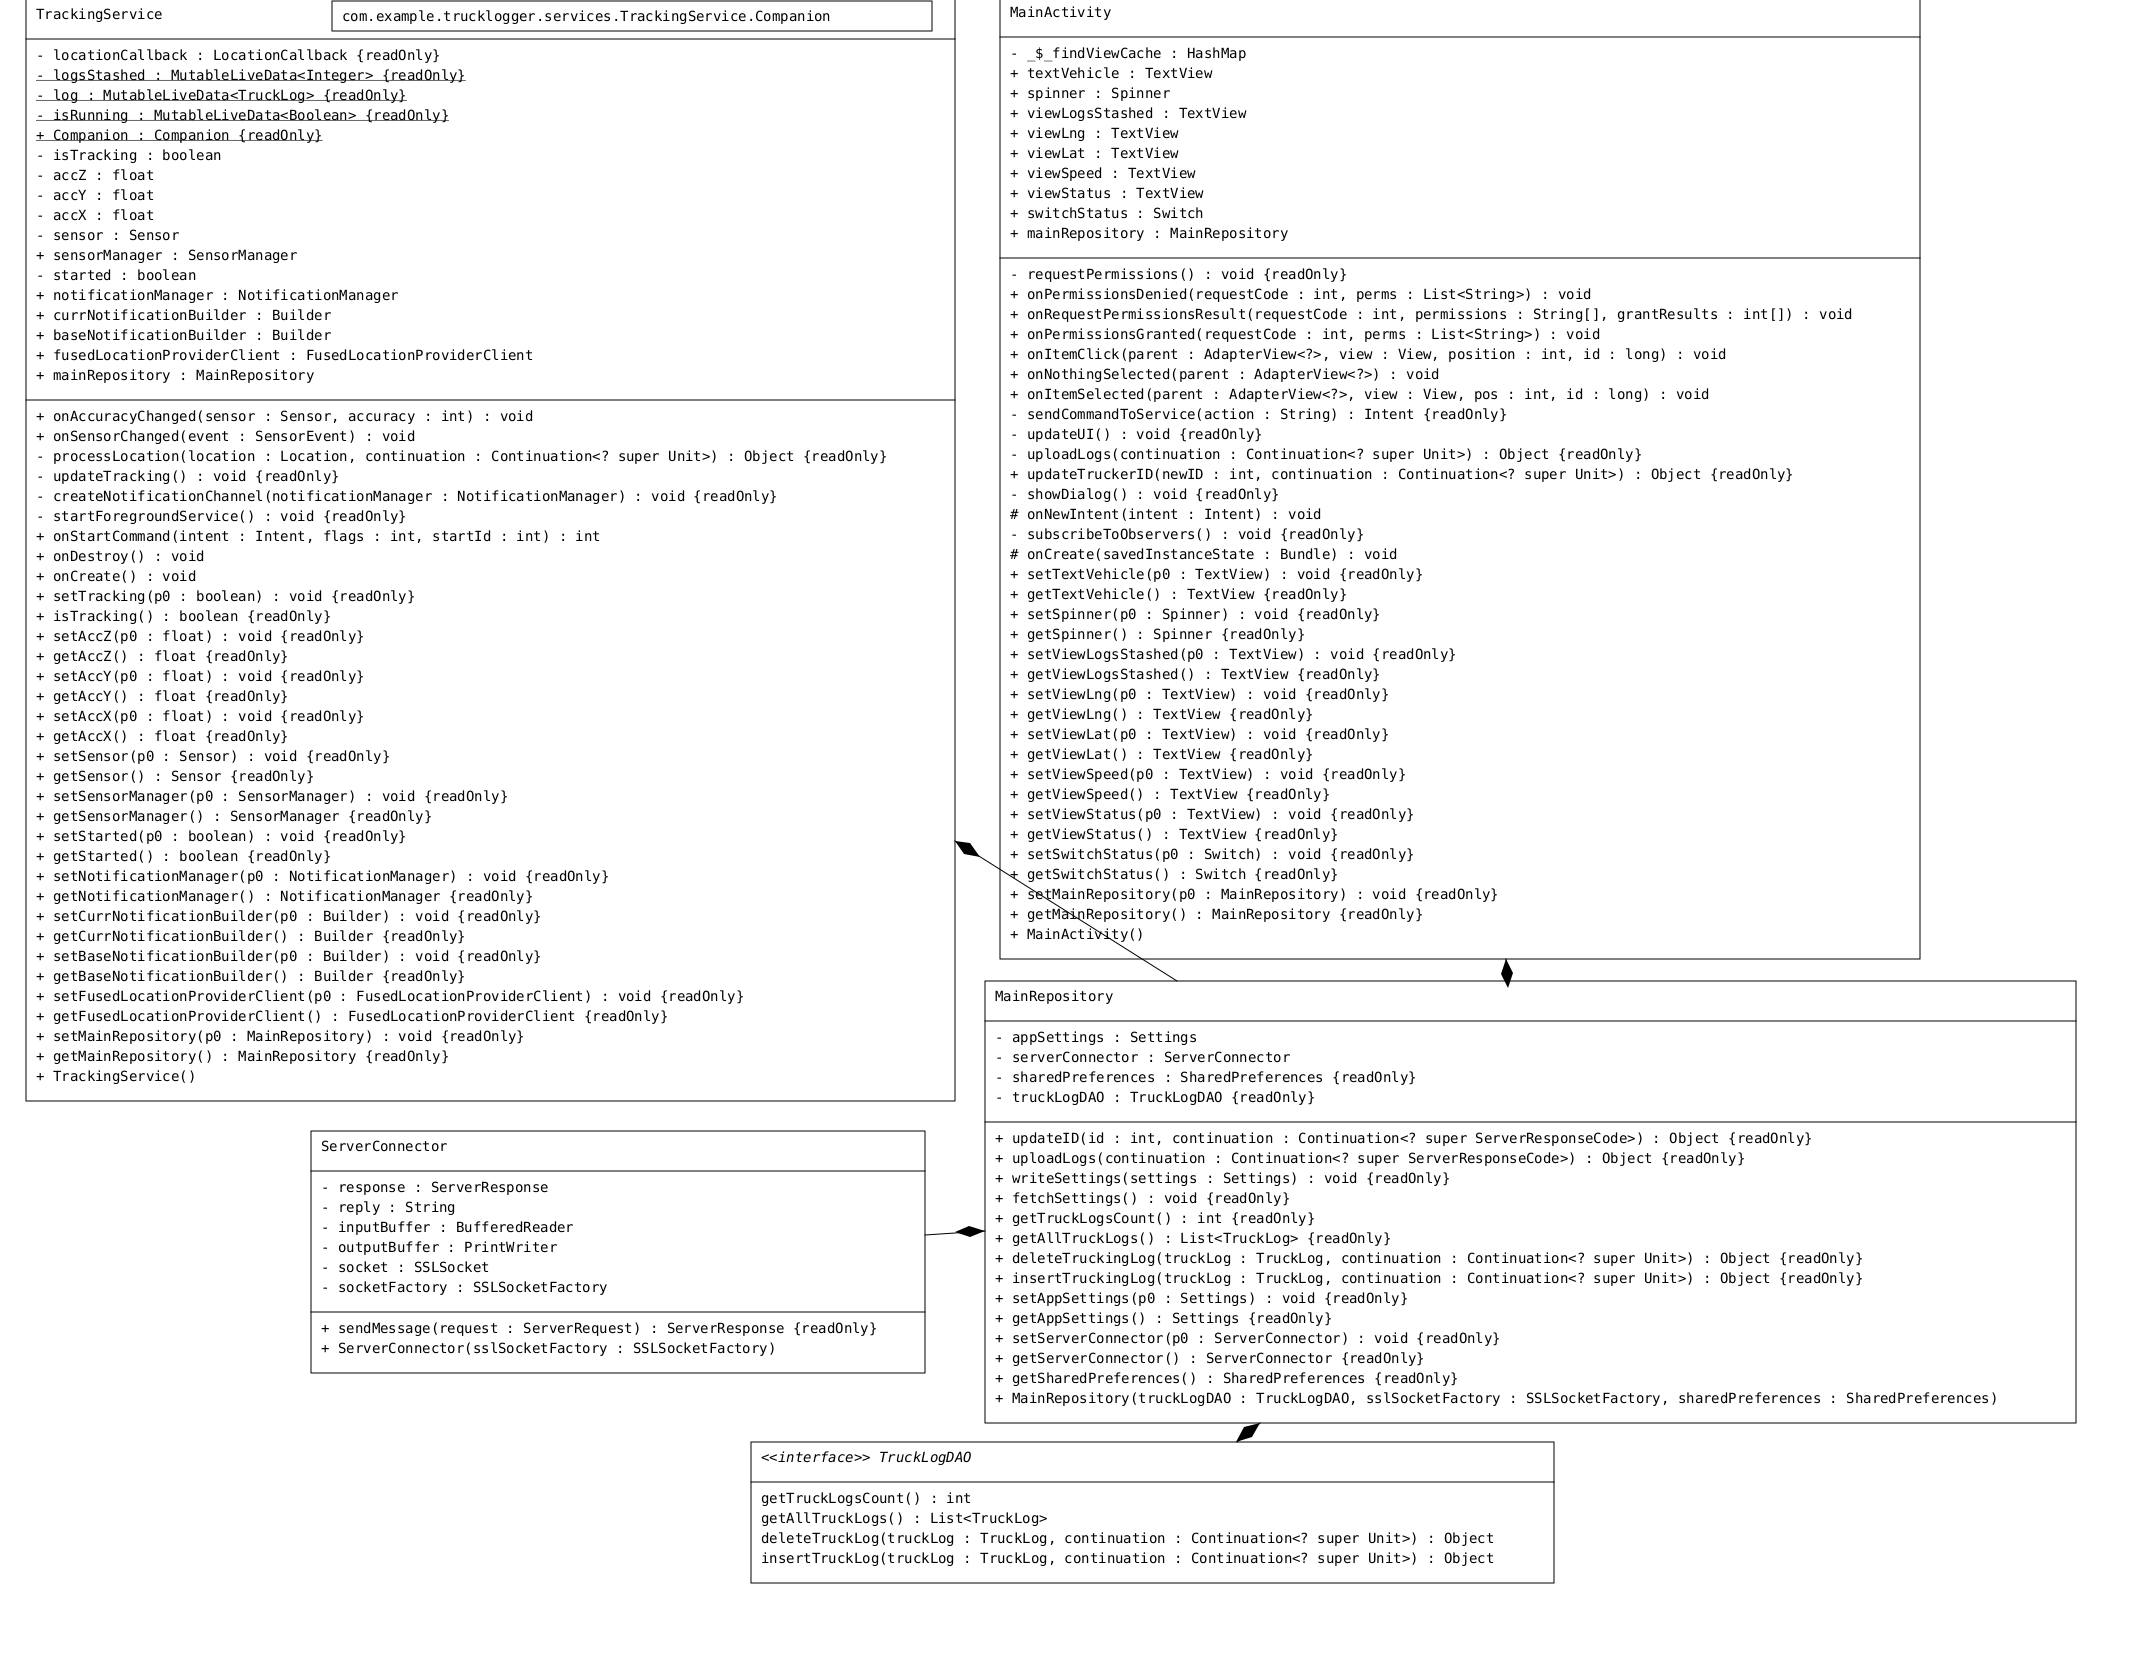
\includegraphics[width=6.5in]{uml_android.png}
\caption{Android Application - Abridged \ac{uml} diagram}
\label{fig:uml_android}
\end{figure}

Figure \ref{fig:uml_android} depicts an abridged generated \ac{uml} diagram of the android source code.
Much detail is omitted for the sake of simplicity.
It is noted that much of the initially planned architecture is successfully implemented.
\pagebreak

\subsection{\ac{io} Server}\label{App:io_server}
\begin{figure}[H]
\centering
    \subfigure[Server]
    {
        \centering
        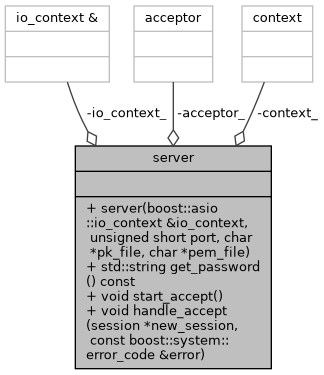
\includegraphics[height=3in]{../diag/io_server.png}
        \label{fig:io_server}
    }
    \subfigure[Session]
    {
        \centering
        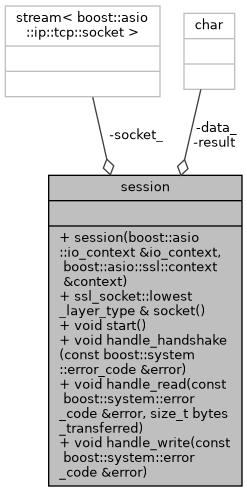
\includegraphics[height=3in]{../diag/io_session.png}
        \label{fig:io_session}
    }\\
    \subfigure[Handler]
    {
        \centering
        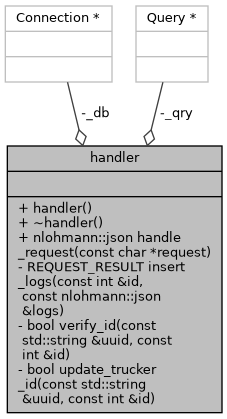
\includegraphics[height=3in]{../diag/io_handler.png}
        \label{fig:io_handler}
    }
\caption{\ac{io} Server - Classes}
\label{fig:uml_io}
\end{figure}

\begin{figure}
\centering
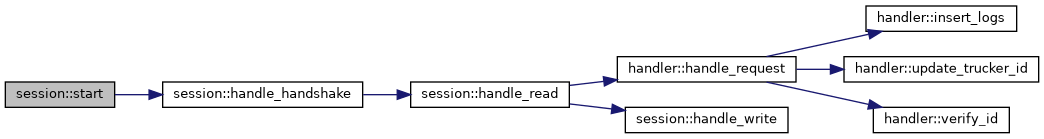
\includegraphics[width=6in]{io_flow.png}
\caption{\ac{io} Server - Functional Flow}
\label{fig:io_flow}
\end{figure}

Figure \ref{fig:uml_io} depicts the class methods implemented in the \ac{io} server.
The server class in figure \ref{fig:io_server} details the server implementation, which assigns a session to an incoming connection.
The session class in figure \ref{fig:io_session} handles the verification procedure required for \ac{ssl}, which includes the handshake, encryption and decryption.
The handler class in figure \ref{fig:io_handler} handles the actual implemented business logic required for operation, including verification, updating \ac{id}s and inserting new log data.

The typical flow (method calling order) of each connection is detailed in \ref{fig:io_flow}.
